\begin{figure}[H]
\newcommand{\wmgd}{1.02\columnwidth}  % width mauna decomp
\newcommand{\hmgd}{3.51cm}  % height mauna decomp
\newcommand{\mdrd}{\grammarfiguresdir/decomposition/11-Feb-03-mauna2003-s}  % mauna decomp results dir
\newcommand{\mbm}{\hspace{-0.2cm}}  % move back
\begin{tabular}{c}
\mbm 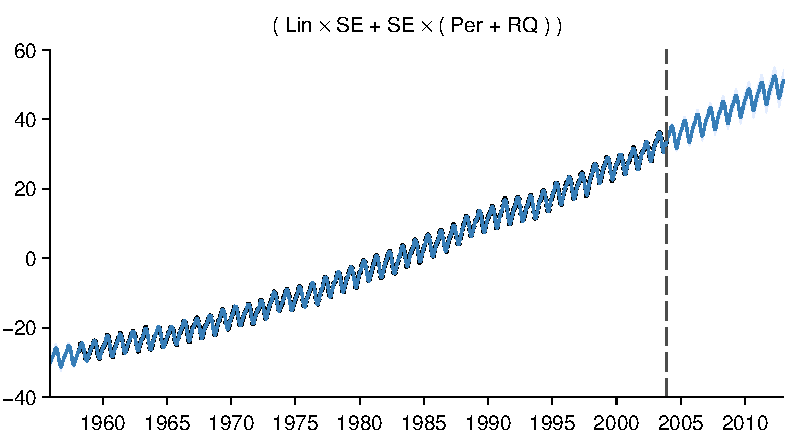
\includegraphics[width=\wmgd,height=\hmgd]{\mdrd/03-mauna2003-s_all} \\ = \\
\mbm 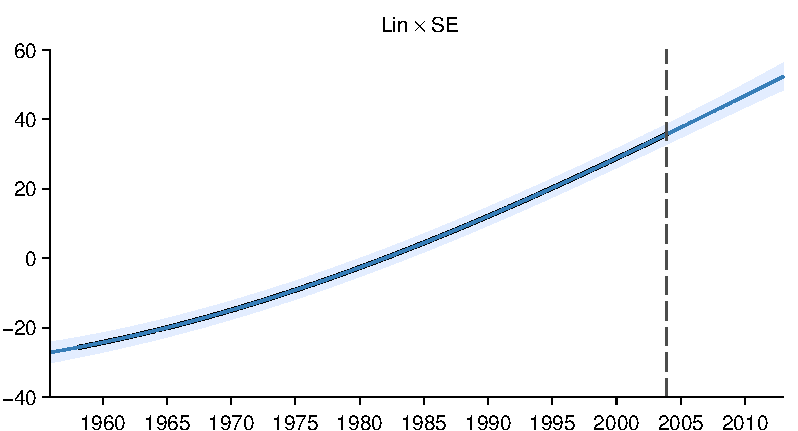
\includegraphics[width=\wmgd,height=\hmgd]{\mdrd/03-mauna2003-s_1} \\ + \\
\mbm 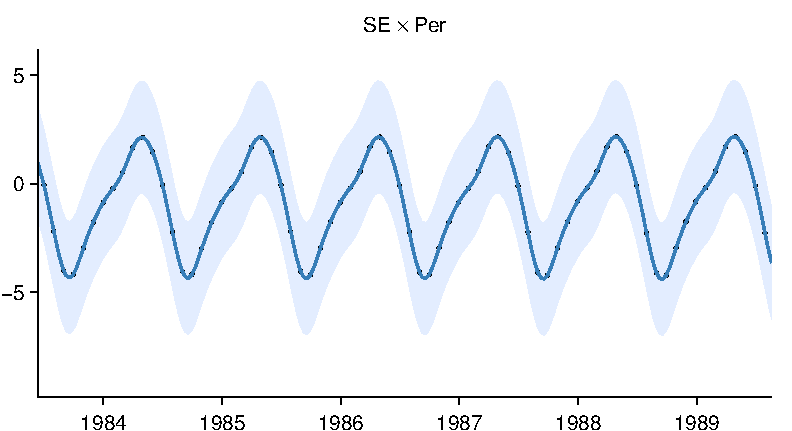
\includegraphics[width=\wmgd,height=\hmgd]{\mdrd/03-mauna2003-s_2_zoom} \\ + \\
\mbm 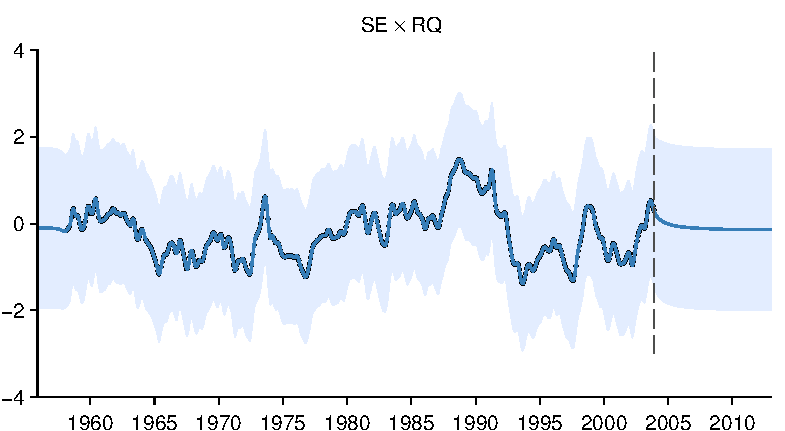
\includegraphics[width=\wmgd,height=\hmgd]{\mdrd/03-mauna2003-s_3} \\ + \\
\mbm 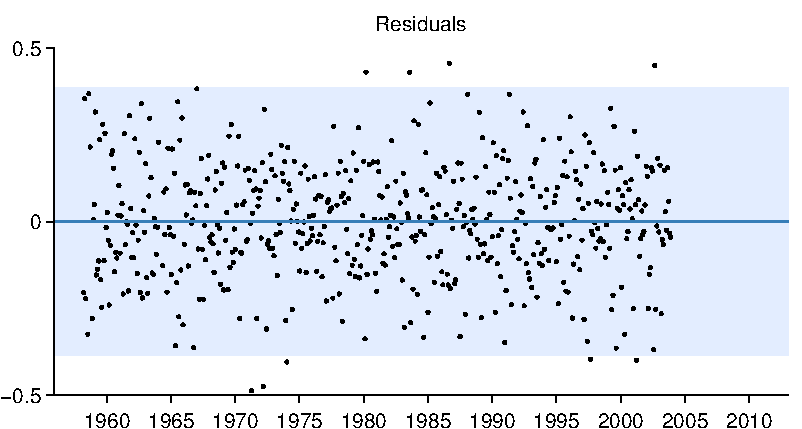
\includegraphics[width=\wmgd,height=\hmgd]{\mdrd/03-mauna2003-s_resid}
\end{tabular}
\caption{First row: The posterior on the Mauna Loa dataset, after a search of depth 10.  Subsequent rows show the automatic decomposition of the time series.  The decompositions shows long-term, yearly periodic, medium-term anomaly components, and residuals, respectively.  In the third row, the scale has been changed in order to clearly show the yearly periodic structure.}
\label{fig:mauna_decomp}
\end{figure}

